\section{Projeto}

\begin{frame}
  \frametitle{Poluição do Ar em Acra, capital de Gana}
  Projeto Internacional: \\
  \textit{Air Pollution in Accra Neighborhoods: Spatial, Socioeconomic, and Temporal Patterns} 
  coordenado por pesquisadores da \textit{Harvard School of Public Healt} nos Estados Unidos
  e da Universidade de Ghana.
\end{frame}

\begin{frame}
 \frametitle{ África Subsariana (SSA)}
  Diferente das cidade dos países desenvolvidos, que tem como principais fontes de poluição 
  a industria e o transporte, nas cidade da SSA as fontes tem outro perfil, pois na SSA:
  \begin{itemize}
    \item população predominantemente rural
    \item muitas vias não pavimentadas
    \item maior taxa de crescimento populacional urbano do mundo
    \item não possuem sistemas de monitoramento sistemático de Poluição do Ar
    \item é comum o uso da queima de biomassa para o cozimento de alimentos (comercial e doméstico), tanto em regiões urbanas quanto rurais.
  \end{itemize}
\end{frame}

\begin{frame}
  \frametitle{Fotos do bairro de Nima}
  \begin{figure}[H]
    \centering
    \caption{Fotos do bairro de Nima}
    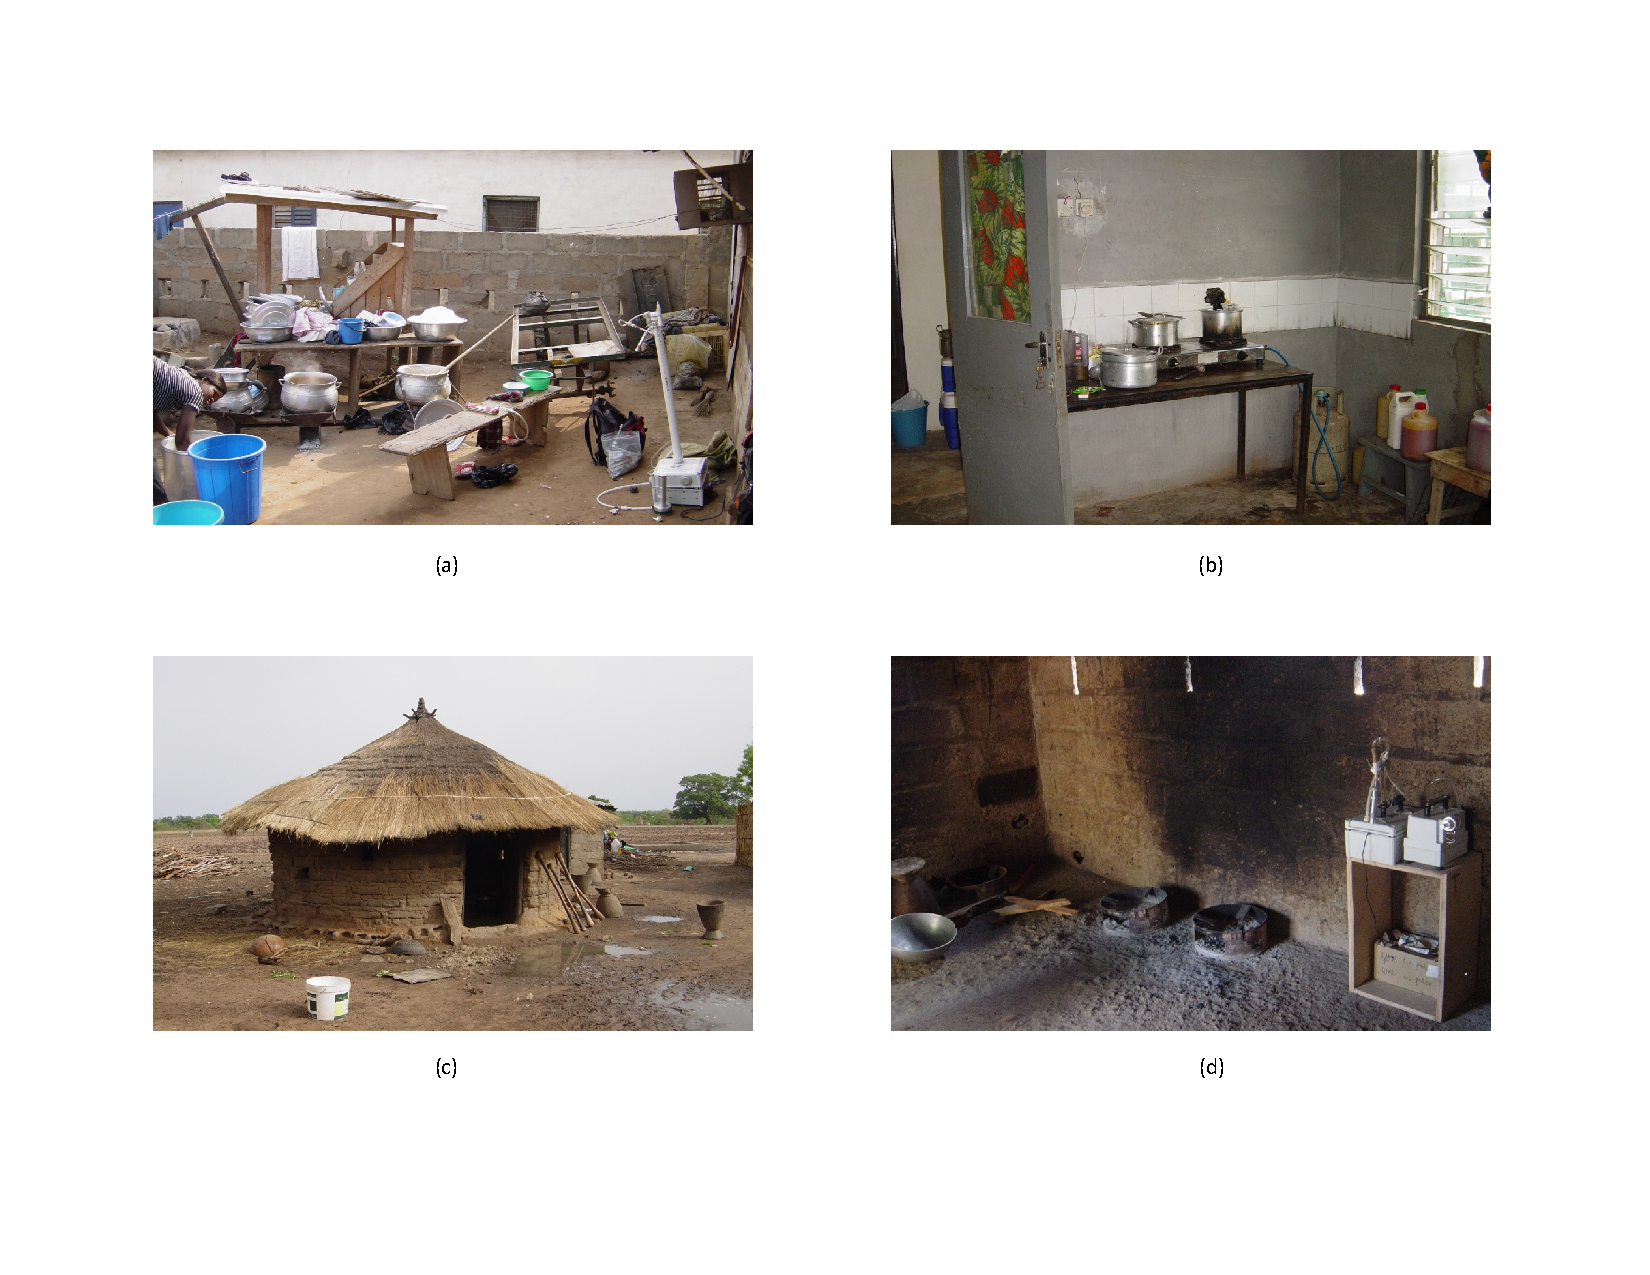
\includegraphics[scale=0.35]{../../../inputs/zheng_images/nima.pdf}
  \end{figure}
\end{frame}

\begin{frame}
  \frametitle{Localização no Mapa}
  \begin{figure}[H]
    \centering
    \caption{Localização no Mapa}
    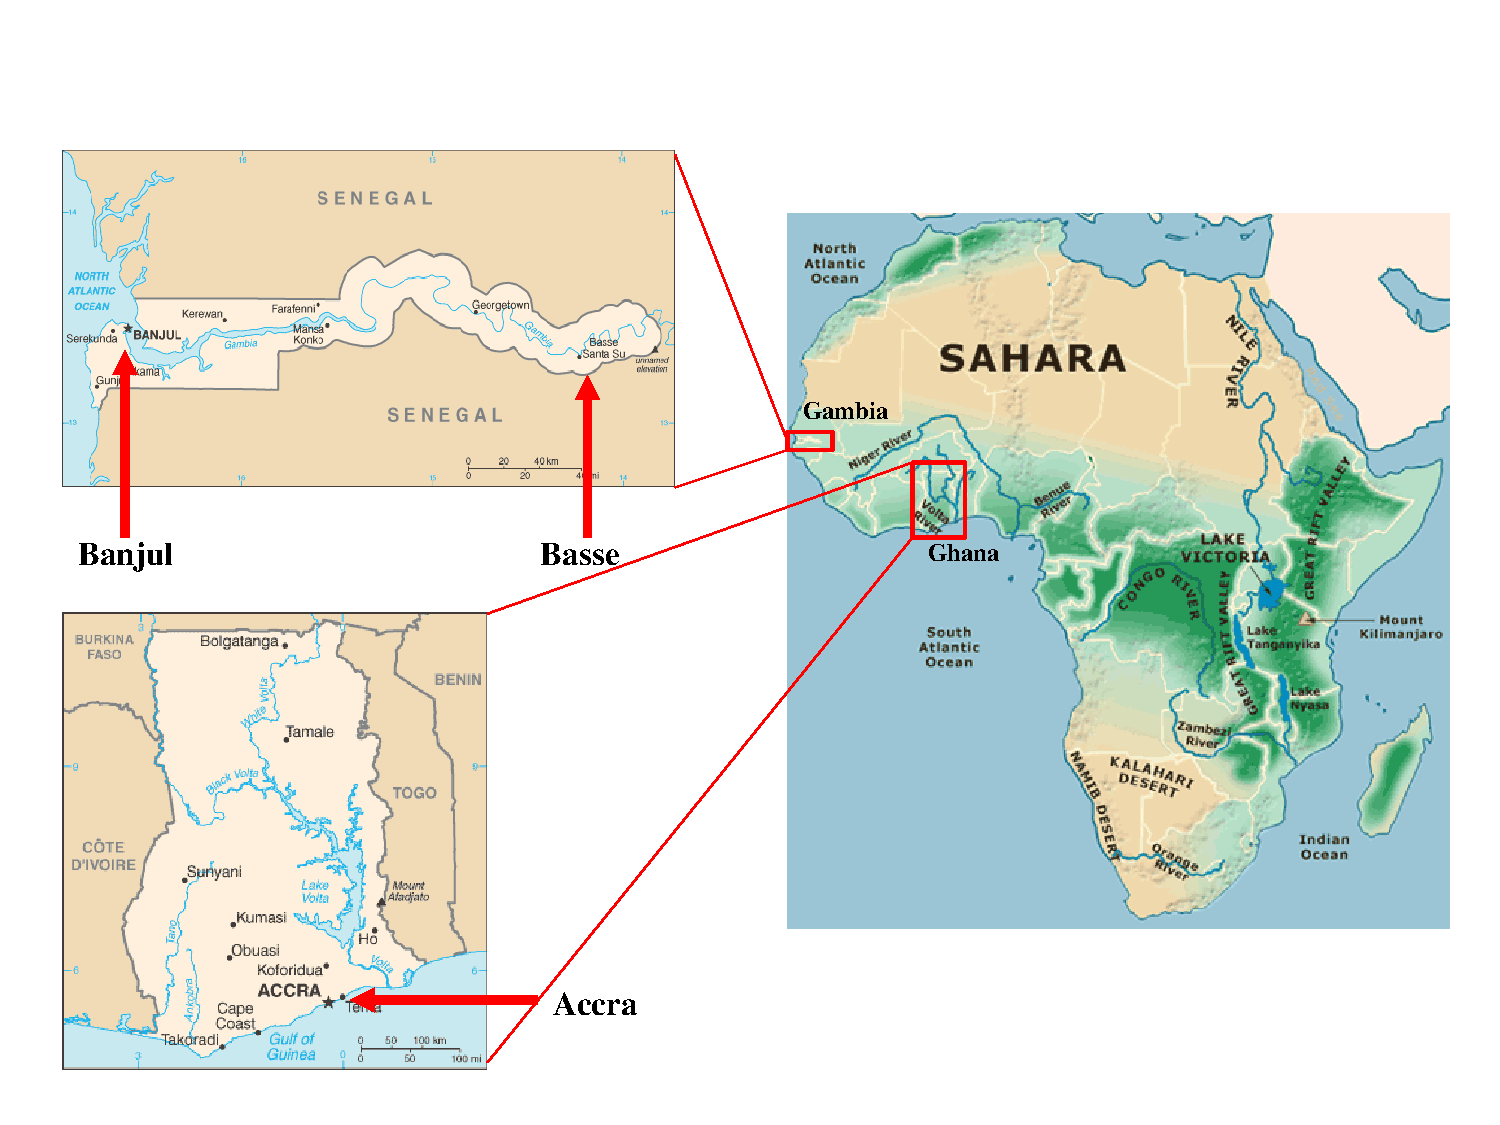
\includegraphics[scale=0.35]{../../../inputs/zheng_images/africa_ghana.pdf}
  \end{figure}
\end{frame}

